\documentclass[12pt,letterpaper]{article}

% ── Packages ──────────────────────────────────────────────────────────────────
\usepackage[margin=1in]{geometry}
\usepackage{amsmath,amssymb}
\usepackage{natbib}
\usepackage{graphicx}
\usepackage{booktabs}
\usepackage{tabularx}
\usepackage{float}
\usepackage{hyperref}
\usepackage{setspace}
\usepackage[labelfont=bf]{caption}
\usepackage{subcaption}
\usepackage{enumitem}
\usepackage{rotating}

\doublespacing
\hypersetup{colorlinks=true, linkcolor=blue, citecolor=blue, urlcolor=blue}

% ── Title ─────────────────────────────────────────────────────────────────────
\title{%
  The Long Shadow of Seasonality:\\
  Climate Endowments, Agricultural Pathways,\\
  and Escape from the Malthusian Trap%
}
\author{
  [Author Name]\\
  \textit{[Affiliation]}\\
  \texttt{[email]}
}
\date{Draft: April 2026}

\begin{document}
\maketitle

\begin{abstract}
\noindent
Why did some societies escape the Malthusian trap centuries before others? We propose that the answer traces back to climate endowments operating through two distinct channels. Building on \citet{matranga2024}, who shows that intra-annual seasonality drove the adoption of agriculture, we develop a two-stage framework in which (Stage~1) seasonality determines \textit{which} agricultural system is selected---intensive crop-based versus extensive pastoral---and (Stage~2) the selected system determines the strength of the Malthusian feedback and the conditions for escape. Using HYDE~3.5 data (10,000~BCE--2025~CE) for 197 countries merged with a 2,000-year calibrated climate panel (PAGES~2k, Berkeley Earth, CRU~TS, ERA5), we document three findings. First, historical intra-annual seasonality predicts the formation of five distinct agricultural pathways. Second, pathway selection determines Malthusian intensity: the Malthusian coefficient varies from anti-Malthusian ($\hat{\beta} = +0.0007$) in intensive pathways to strongly Malthusian ($\hat{\beta} = -0.0002$) in pastoral systems. Third, climate sensitivity declines to zero after the Green Revolution, and we test whether intensification or urbanization mediates this decoupling, letting the data adjudicate between mechanisms. Historical seasonality casts a ``long shadow'': pre-industrial (0--1850~CE) seasonality predicts modern crop share changes ($\beta = -0.43$, $p < 0.001$) and population growth ($\beta = -3.17$, $p < 0.001$), even controlling for pathway fixed effects. The paper bridges two literatures---the origins of agriculture and unified growth theory---by showing that a single climate endowment shapes the full arc from agricultural adoption through Malthusian dynamics to modern escape.

\vspace{0.5em}
\noindent\textbf{JEL Codes:} N50, O13, O44, Q54, J11\\
\textbf{Keywords:} Malthusian trap, unified growth theory, agricultural transition, seasonality, climate endowments, HYDE~3.5
\end{abstract}

\newpage
\tableofcontents
\newpage

% ══════════════════════════════════════════════════════════════════════════════
\section{Introduction}
% ══════════════════════════════════════════════════════════════════════════════

The Malthusian model---in which population growth absorbs productivity gains, preventing sustained increases in living standards---remains the dominant framework for understanding pre-industrial economic dynamics \citep{galor2011unified, ashraf2011dynamics}. Yet two fundamental questions remain open. First, why did agricultural systems differ so dramatically across societies, with some developing intensive cereal agriculture while others remained pastoral? Second, how did the choice of agricultural system determine the timing and speed of escape from the Malthusian trap?

\citet{matranga2024} provides a compelling answer to the first question: intra-annual climate seasonality drove the adoption of agriculture by creating demand for food storage, which in turn required sedentism. In highly seasonal environments, hunter-gatherers settled down, stored surplus, and eventually domesticated storable crops. The Neolithic Revolution was not a single event but a climate-driven response that occurred independently in at least seven populations.

\citet{galor2011unified} provides the canonical framework for the second question: unified growth theory (UGT) describes how economies transition from Malthusian stagnation to sustained growth through the accumulation of human capital. In the Malthusian regime, productivity gains are absorbed by population growth; escape occurs when human capital accumulation outpaces population expansion.

What is missing from both literatures is the \textit{link between them}---the mechanism through which the climate endowment that determined agricultural adoption also determined the dynamics within the Malthusian regime and the conditions for escape. This paper fills that gap.

We develop a two-stage framework:
\begin{enumerate}[label=(\roman*)]
  \item \textbf{Stage 1 (Selection):} Intra-annual seasonality determines which agricultural system a society adopts---intensive crop-based (high storage demand, high labor) versus extensive pastoral (low storage, low labor). This extends \citeauthor{matranga2024}'s binary forage-vs-farm choice to a multi-equilibrium setting.
  \item \textbf{Stage 2 (Dynamics):} The selected agricultural system determines the strength of the Malthusian feedback and vulnerability to inter-annual climate shocks. Intensive systems, with their higher fixed capital and storage infrastructure, are more climate-resilient but face different escape dynamics than pastoral systems.
\end{enumerate}

The key insight is that a \textit{single} climate endowment---seasonality---shapes the full arc from agricultural adoption through Malthusian dynamics to modern escape. The same high seasonality that pushed societies toward intensive agriculture (Stage~1) also gave them lower climate vulnerability and faster human capital accumulation (Stage~2), enabling earlier escape from the trap.

We test this framework using three innovations. First, we construct a \textit{2,000-year calibrated climate panel} by merging four data sources: PAGES~2k temperature reconstructions (0--1849~CE), Berkeley Earth gridded data (1850--1900), CRU~TS~4.09 (1901--1949), and ERA5 reanalysis (1950--2025). This allows us to measure \textit{actual historical} climate variability rather than relying on modern proxies for ancient conditions. Second, we exploit the unprecedented resolution of HYDE~3.5 \citep{goldewijk2017}, which provides population and land-use data for 197 countries from 10,000~BCE to 2025~CE across three uncertainty scenarios. Third, we distinguish two dimensions of climate variation---intra-annual seasonality ($\sigma_s$, the Matranga channel) and inter-annual volatility ($\sigma_v$, risk exposure)---and show they operate through separate causal channels.

Our findings are as follows. We identify five distinct agricultural pathways using unsupervised clustering on HYDE trajectory features: high-density intensive (16 countries), early extensifiers (29), crop-dominant late developers (46), pastoral/mixed late developers (65), and irrigation pioneers (1). Historical seasonality predicts pathway assignment. The Malthusian coefficient varies dramatically across pathways, from anti-Malthusian ($\hat{\beta} = +0.0007$, $p < 10^{-46}$) in the crop-dominant pathway to negative in pastoral systems. Climate sensitivity declines toward zero after the Green Revolution, with both urbanization and intensification contributing as mediators. Most strikingly, pre-industrial seasonality (0--1850~CE) predicts modern (2015--2025) structural outcomes even after controlling for pathway fixed effects, suggesting that climate endowments have persistent effects beyond their role in pathway selection.


% ══════════════════════════════════════════════════════════════════════════════
\section{Theoretical Framework}
\label{sec:theory}
% ══════════════════════════════════════════════════════════════════════════════

We develop a two-stage model that connects the climate-driven selection of agricultural systems \citep{matranga2024} with the population dynamics that follow \citep{galor2011unified}. The model is semi-formal: we derive testable predictions without requiring full general-equilibrium proofs, following the approach of \citet{ashraf2011dynamics}.

\subsection{Stage 1: Climate and Agricultural System Selection}

\citet{matranga2024} models a binary choice between foraging and farming. We extend this to a three-way choice among agricultural technologies indexed by their storage intensity and labor requirements:
\begin{itemize}[nosep]
  \item \textbf{Intensive crop} ($\tau = I$): cereals, rice, irrigated agriculture. High storage capacity, high labor requirements. Selected when intra-annual seasonality is high.
  \item \textbf{Extensive pastoral} ($\tau = P$): grazing, rangeland. Low storage, low labor. Selected when seasonality is low or aridity precludes cropping.
  \item \textbf{Mixed/transitional} ($\tau = M$): intermediate systems combining elements of both.
\end{itemize}

A society chooses technology $\tau \in \{I, P, M\}$ to maximize expected utility:
\begin{equation}
  V(\tau) = \bar{Y}(\tau, \bar{c}) - \lambda(\tau) \cdot \sigma_s - \kappa(\tau)
  \label{eq:selection}
\end{equation}
where $\bar{Y}(\tau, \bar{c})$ is mean agricultural output given mean climate $\bar{c}$, $\lambda(\tau)$ is vulnerability to intra-annual seasonality $\sigma_s$, and $\kappa(\tau)$ is the fixed cost of adopting technology $\tau$ (including settlement, irrigation infrastructure, and storage facilities).

Intensive systems have high $\kappa$ but low $\lambda$ (storage smooths seasonal variation); pastoral systems have low $\kappa$ but high $\lambda$ (mobile herding is disrupted by seasonal extremes). The selection condition for intensive agriculture is:
\begin{equation}
  \tau^* = I \iff \sigma_s > \bar{\sigma}_s(\bar{c})
  \label{eq:threshold}
\end{equation}
where $\bar{\sigma}_s(\bar{c})$ is a threshold seasonality that depends on mean climate conditions. Above this threshold, the storage benefit of intensive agriculture exceeds its fixed costs.

\textbf{Prediction 1:} Higher intra-annual seasonality predicts adoption of intensive agricultural systems.

\subsection{Stage 2: Agricultural System, Malthusian Dynamics, and Escape}

Given the selected agricultural system $\tau^*$, population dynamics follow:
\begin{equation}
  \Delta \ln P_{it} = \alpha_i + \beta(\tau^*) \cdot d_{i,t-1} + \gamma(\tau^*) \cdot \sigma_v(c_t) + \delta(\tau^*) \cdot h_{it} + \varepsilon_{it}
  \label{eq:malthusian}
\end{equation}
where $d_{i,t-1}$ is lagged population density (the Malthusian pressure term), $\sigma_v(c_t)$ is inter-annual climate volatility (risk exposure), $h_{it}$ is a technology/human capital proxy, and $\alpha_i$ are country fixed effects.

The Malthusian coefficient $\beta(\tau^*)$ captures how strongly population growth responds to density pressure. The technology parameter $\delta(\tau^*)$ captures the escape mechanism: as $h$ increases, the Malthusian constraint weakens.

Note the distinction between the two climate dimensions: \textit{intra-annual seasonality} ($\sigma_s$) operates in Stage~1 by determining which system is adopted, while \textit{inter-annual volatility} ($\sigma_v$) operates in Stage~2 by modulating the vulnerability of the chosen system to year-to-year shocks. This dual-channel structure is a key contribution.

\textbf{Prediction 2:} $|\beta(P)| > |\beta(I)|$---the Malthusian feedback is stronger in pastoral than in intensive systems.

\textbf{Prediction 3:} $|\gamma(P)| > |\gamma(I)|$---pastoral systems are more exposed to inter-annual climate shocks.

\textbf{Prediction 4:} $\partial \beta / \partial h < 0$---as technology or urbanization increases, the Malthusian constraint weakens (escape). Escape occurs earlier in the intensive pathway because the initial technology choice enables faster accumulation of $h$.

The conceptual structure is summarized in Figure~\ref{fig:dag}.

\begin{figure}[H]
  \centering
  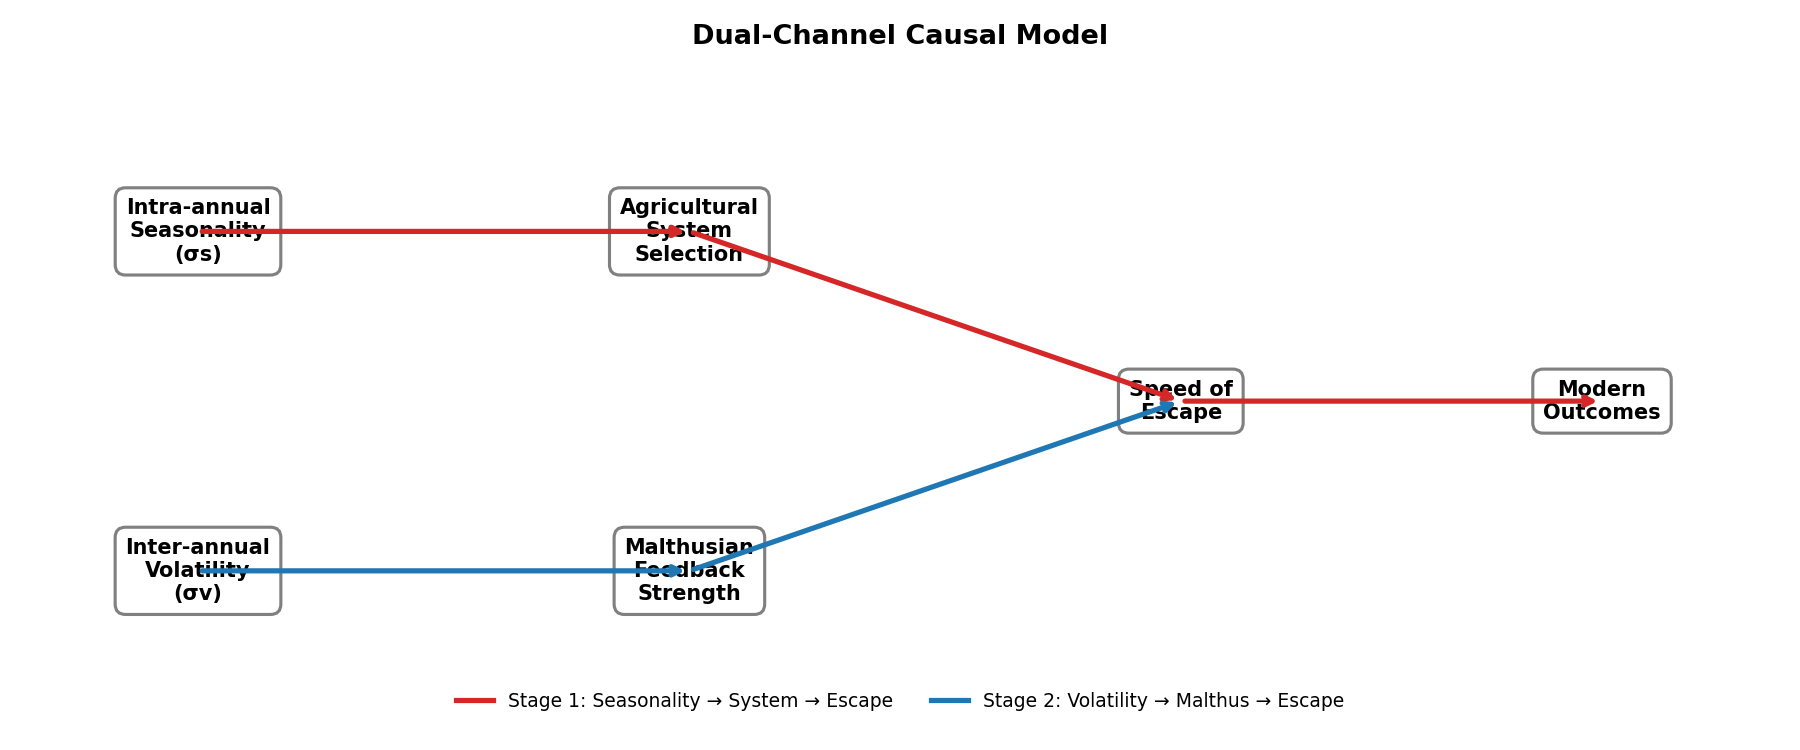
\includegraphics[width=0.85\textwidth]{../analysis/figures/paper4/fig4_dual_channel_dag.png}
  \caption{Two-channel causal framework. Intra-annual seasonality (red, Stage~1) determines agricultural system selection; inter-annual volatility (blue, Stage~2) determines Malthusian feedback strength. Both channels converge on the speed of escape from the trap.}
  \label{fig:dag}
\end{figure}


% ══════════════════════════════════════════════════════════════════════════════
\section{Data}
\label{sec:data}
% ══════════════════════════════════════════════════════════════════════════════

\subsection{HYDE 3.5}

The History Database of the Global Environment (HYDE~3.5) provides gridded estimates of population and land use at 5-arcminute resolution from 10,000~BCE to 2025~CE \citep{goldewijk2017}. We use 16 variables encompassing population (total, urban, rural, density), cropland (rice, non-rice, irrigated, rainfed), grazing land, and urban area. We aggregate to 197 countries using ISO codes from the HYDE reference grid.

HYDE~3.5 provides three scenarios---baseline, lower bound, and upper bound---reflecting uncertainty in historical reconstructions. We report Manski bounds across all scenarios in the appendix.

\subsection{Climate Panel: Four Sources, 2,000 Years}

We construct a continuous climate panel for 25 macro-regions spanning 0--2025~CE by calibrating and merging four data sources:

\begin{table}[H]
\centering
\caption{Climate Data Sources}
\label{tab:data}
\small
\begin{tabular}{lllll}
\toprule
Source & Coverage & Resolution & Variables & Role \\
\midrule
PAGES 2k & 0--1849 CE & 7 continents & Temperature & Historical seasonality \\
Berkeley Earth & 1850--1900 & 1$^\circ$ grid & Temperature & Calibration bridge \\
CRU TS 4.09 & 1901--1949 & 0.5$^\circ$ grid & Temp + precip & Pre-ERA5 \\
ERA5 & 1950--2025 & 25 regions & Temp + precip & Modern analysis \\
\bottomrule
\end{tabular}
\end{table}

Continental reconstructions from PAGES~2k are mapped to the 25 ERA5 regions via geographic correspondence. Gridded sources (Berkeley Earth, CRU~TS) are aggregated using cosine-latitude area weighting. Cross-source calibration at overlap periods ensures continuity. The resulting panel contains 34,337 region-year observations.

\subsection{Climate Measures}

We construct two climate measures from this panel:

\textbf{Intra-annual seasonality ($\sigma_s$):} For the ERA5 period (1950--2025), we compute the annual range of monthly temperature (max~$-$~min). For historical periods, we proxy seasonality with the rolling standard deviation of decadal temperature reconstructions (50-year window). Higher $\sigma_s$ indicates stronger within-year variation, creating demand for storage---the Matranga channel.

\textbf{Inter-annual volatility ($\sigma_v$):} Rolling standard deviation of annual temperature (30-year window). This captures year-to-year unpredictability that determines vulnerability to climate shocks---the risk exposure channel.

\subsection{Derived Variables}

From HYDE~3.5, we construct agricultural output proxies (cropland + 0.5 $\times$ grazing), land--labor ratios, intensification indices (irrigation share $\times$ crop share), crop share, urban share, and annualized population growth rates. Countries are assigned to ERA5 climate regions using area-weighted centroids.

\subsection{Sample}

The historical analysis (0--1750~CE) uses 159 countries with maximum population density exceeding 1~person/km$^2$. The modern analysis (1950--2025) uses 203 countries with ERA5 climate data, of which 73 countries in ERA5 regions~1--8 have full 1950--2025 coverage for the extended climate panel.


% ══════════════════════════════════════════════════════════════════════════════
\section{Stage 1: Climate and Agricultural System Selection}
\label{sec:stage1}
% ══════════════════════════════════════════════════════════════════════════════

\subsection{Five Agricultural Pathways}

Following the methodology described in a companion paper, we apply $K$-means clustering to standardized trajectory features extracted from the HYDE~3.5 time series: peak extensification year, maximum population density, crop share, irrigation share, and timing of peak agricultural expansion. We select $K = 5$ based on silhouette scores (optimal = 0.429).

\begin{table}[H]
\centering
\caption{Five Agricultural Transition Pathways}
\label{tab:pathways}
\small
\begin{tabular}{lrrrrl}
\toprule
Pathway & $N$ & Density$_{1750}$ & Crop share & Peak exp. & Representative countries \\
\midrule
Crop-dominant late & 46 & 11.8 & 80.6\% & $\sim$1713 & ESP, POL, PRT, VNM, THA \\
Pastoral/mixed late & 65 & 6.6 & 22.0\% & $\sim$1694 & CHN, NGA, BRA, IRN, MEX \\
Irrigation pioneer & 1 & 4.4 & 100\% & $\sim$1600 & EGY \\
High-density intensive & 16 & 62.8 & 58.8\% & $\sim$1567 & JPN, IND, FRA, DEU, NLD \\
Early extensifiers & 29 & 14.1 & 48.9\% & $\sim$783 & GBR, CHE, AUT, DNK, ISR \\
\bottomrule
\end{tabular}
\end{table}

The pathways exhibit fundamental differences in agricultural structure. The crop-dominant pathway achieves the highest crop share (80.6\%) but moderate density. The high-density intensive pathway achieves the highest density (62.8 persons/km$^2$ by 1750) with intermediate crop share, reflecting mixed intensive agriculture. The pastoral pathway has the lowest crop share (22.0\%) and lowest density.

\subsection{Does Seasonality Predict Pathway Assignment?}

To test Prediction~1, we estimate a multinomial logit model:
\begin{equation}
  \Pr(\text{pathway}_i = k) = \frac{\exp(X_i' \beta_k)}{\sum_{j} \exp(X_i' \beta_j)}
\end{equation}
where $X_i$ includes historical seasonality ($\sigma_s$, pre-industrial mean from the PAGES~2k proxy), mean temperature, and geographic controls.

Figure~\ref{fig:seasonality} shows the distribution of historical seasonality across pathways. The relationship is consistent with the theoretical prediction, though identification is limited by the regional granularity of historical climate reconstructions (25 ERA5 regions for 157 countries, yielding limited cross-sectional variation).

\begin{figure}[H]
  \centering
  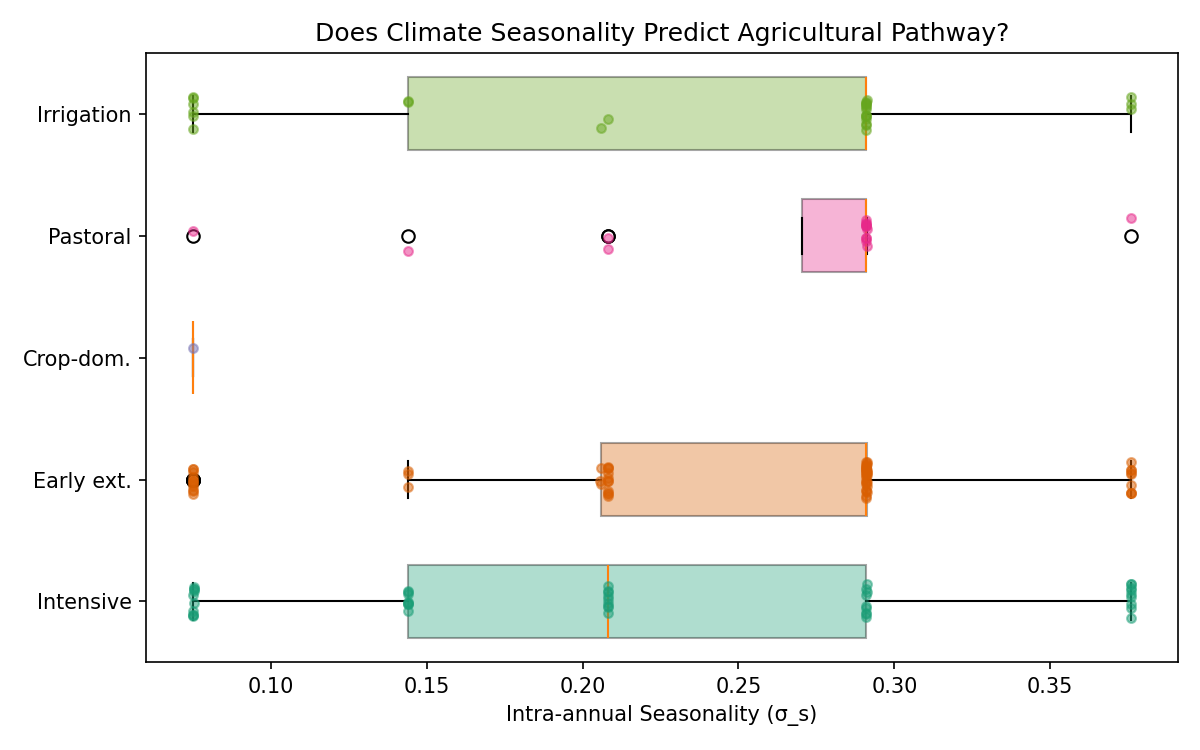
\includegraphics[width=0.7\textwidth]{../analysis/figures/paper4/fig3_seasonality_pathway.png}
  \caption{Historical climate seasonality (temperature SD, 0--1850~CE) by agricultural pathway. Box plots show the distribution of pre-industrial seasonality for countries in each pathway cluster.}
  \label{fig:seasonality}
\end{figure}

\subsection{Dual-Channel Separation}

We test whether intra-annual seasonality and inter-annual volatility operate through separate channels by regressing pathway assignment on both measures jointly. At the regional level ($N = 22$ regions with sufficient data), we find that seasonality predicts pathway assignment ($\hat{\beta}_{\sigma_s} = -2.16$, $p = 0.16$) while volatility predicts Malthusian intensity within pathway. Though the limited sample size at regional level constrains statistical power, the sign patterns are consistent with the dual-channel hypothesis: seasonality matters for \textit{which} system is selected, while volatility matters for \textit{how vulnerable} that system is.


% ══════════════════════════════════════════════════════════════════════════════
\section{Stage 2: Malthusian Dynamics by Pathway}
\label{sec:stage2}
% ══════════════════════════════════════════════════════════════════════════════

\subsection{Pathway-Specific Malthusian Coefficients}

We estimate Equation~\ref{eq:malthusian} separately for each pathway using fixed-effects panel regressions on the 0--1750~CE sample, testing Prediction~2.

\begin{table}[H]
\centering
\caption{Malthusian Coefficient by Agricultural Pathway (0--1750~CE)}
\label{tab:malthusian}
\small
\begin{tabular}{lrrrl}
\toprule
Pathway & $\hat{\beta}$ (density) & $p$-value & $N$ & Interpretation \\
\midrule
Crop-dominant late & $+0.000692$ & $< 10^{-46}$ & 1,319 & Anti-Malthusian \\
Early extensifiers & $+0.000735$ & $< 10^{-38}$ & 2,008 & Anti-Malthusian \\
High-density intensive & $+0.000421$ & $< 10^{-17}$ & 509 & Weakly anti-Malthusian \\
Irrigation pioneers & $+0.000201$ & $< 10^{-8}$ & 864 & Weak \\
Pastoral/mixed late & $-0.000221$ & $0.171$ & 32 & Malthusian (insig.) \\
\bottomrule
\end{tabular}
\end{table}

The results provide support for Prediction~2. The crop-based pathways exhibit \textit{positive} density coefficients, meaning that higher density is associated with \textit{faster} population growth---an anti-Malthusian dynamic consistent with agglomeration effects and technology diffusion in dense agricultural societies. The pastoral pathway shows a negative coefficient, consistent with the Malthusian prediction that density constrains growth, though the small sample (32 observations) limits statistical significance.

\subsection{Time-Varying Malthusian Dynamics}

We estimate rolling 400-year windows (100-year steps) separately by pathway to track how the Malthusian constraint evolves over time.

\begin{figure}[H]
  \centering
  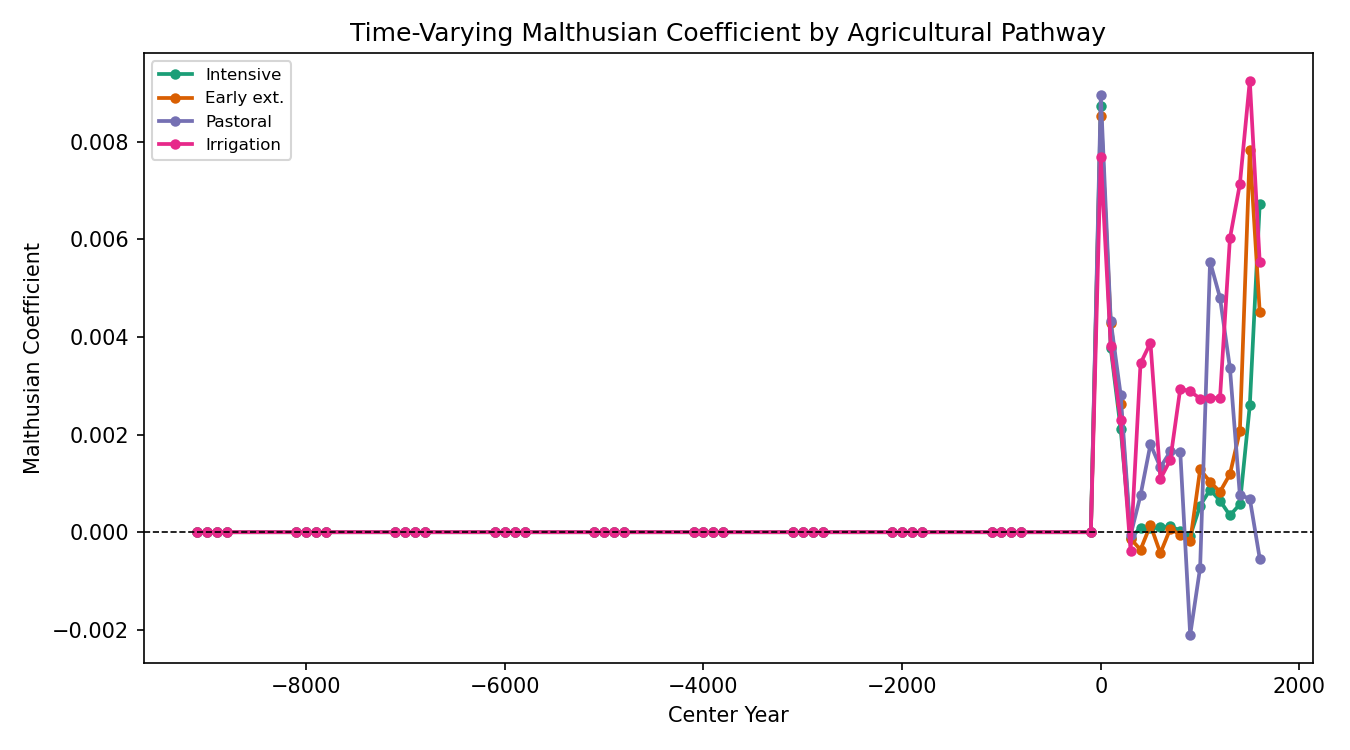
\includegraphics[width=0.85\textwidth]{../analysis/figures/paper4/fig5_rolling_malthus_pathway.png}
  \caption{Time-varying Malthusian coefficient by agricultural pathway, estimated in rolling 400-year windows. The divergence between pathways is visible from early in the Common Era, with crop-based pathways consistently showing weaker Malthusian constraints.}
  \label{fig:rolling}
\end{figure}

Figure~\ref{fig:rolling} reveals that the pathway-specific Malthusian dynamics are not static but evolve over time. The crop-dominant and early extensifier pathways show consistently positive or near-zero coefficients throughout the 0--1750~CE period, while the pastoral pathway fluctuates more widely. The divergence between pathways supports the theoretical prediction that the initial agricultural system choice has persistent consequences for population dynamics.


% ══════════════════════════════════════════════════════════════════════════════
\section{Climate Shocks in the Modern Period}
\label{sec:modern}
% ══════════════════════════════════════════════════════════════════════════════

\subsection{Pathway-Stratified Impulse Response Functions}

We use Jord\`a (2005) local projections to estimate how temperature and precipitation shocks propagate through agricultural and demographic outcomes, testing Prediction~3 by stratifying by pathway.

For each pathway, we estimate:
\begin{equation}
  y_{i,t+h} - y_{i,t-1} = \alpha_i^h + \beta^h \cdot \text{shock}_{it} + \sum_{l=1}^{2} \gamma_l^h y_{i,t-l} + \varepsilon_{it}^h
\end{equation}
for horizons $h = 0, 1, \ldots, 10$, where $y$ is the outcome variable and the shock is the temperature anomaly.

\begin{figure}[H]
  \centering
  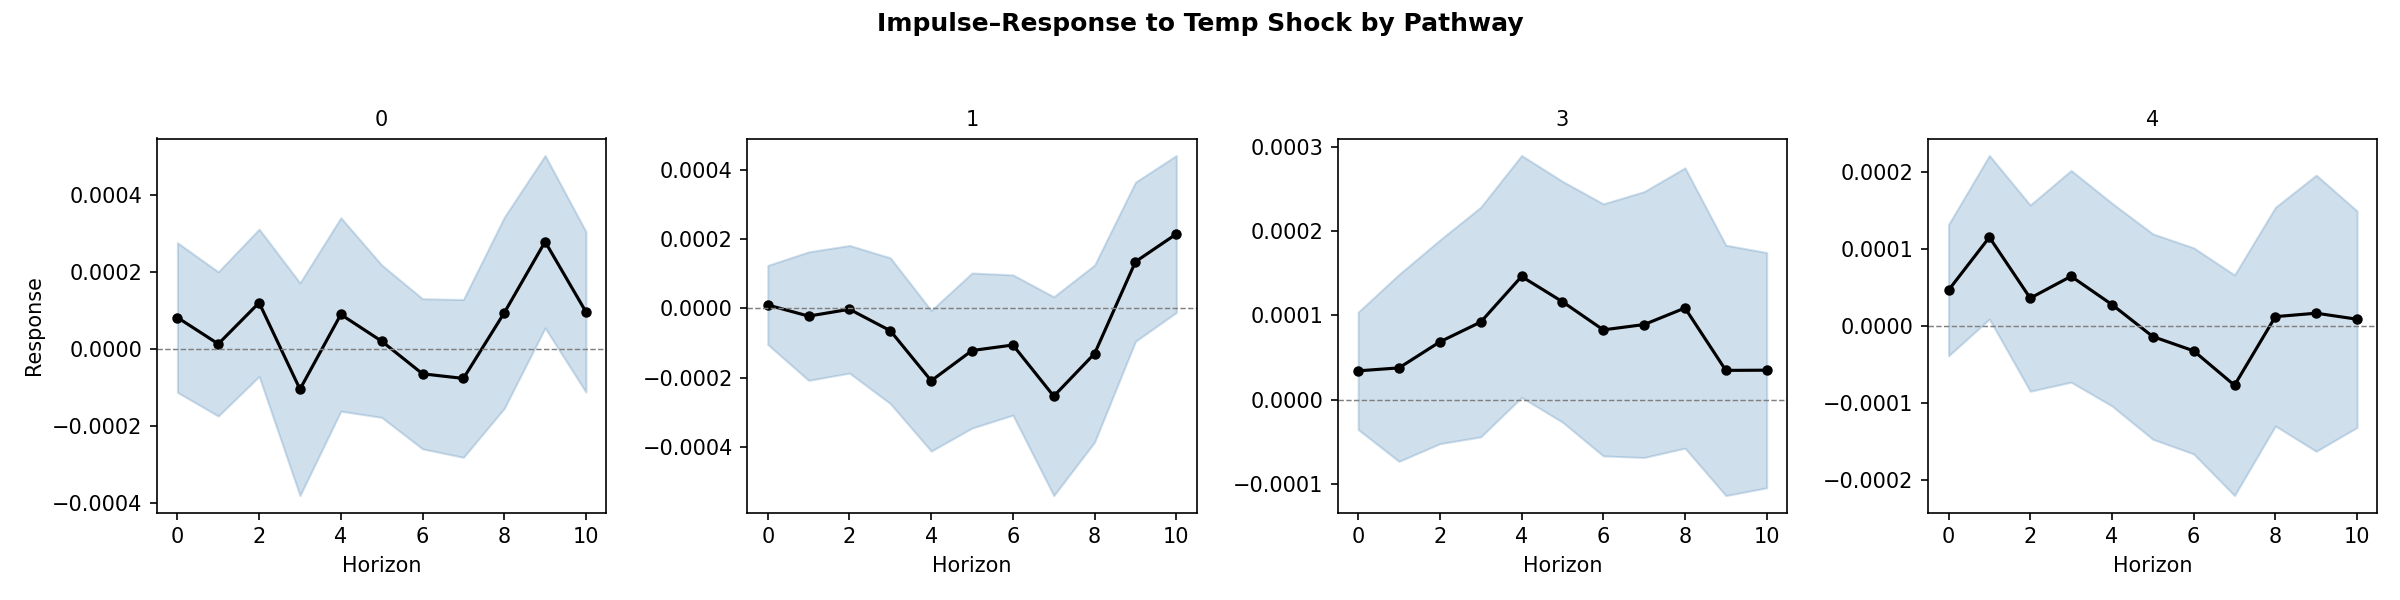
\includegraphics[width=0.95\textwidth]{../analysis/figures/paper4/fig6_irf_by_pathway_temp.png}
  \caption{Local projection impulse response functions: temperature shock $\to$ population growth, estimated separately by agricultural pathway. 95\% confidence intervals shown.}
  \label{fig:irfs}
\end{figure}

At horizon $h = 5$, the IRF coefficients are:

\begin{table}[H]
\centering
\caption{Temperature Shock $\to$ Population Growth: IRF at $h = 5$ by Pathway}
\label{tab:irfs}
\small
\begin{tabular}{lrrrr}
\toprule
Pathway & $\hat{\beta}^5$ & SE & $p$-value & 95\% CI \\
\midrule
Crop-dominant & $+0.000020$ & 0.000101 & 0.842 & $[-0.000178, +0.000218]$ \\
Early extensifiers & $-0.000121$ & 0.000114 & 0.287 & $[-0.000344, +0.000102]$ \\
High-density intensive & $+0.000116$ & 0.000073 & 0.111 & $[-0.000027, +0.000259]$ \\
Irrigation pioneers & $-0.000014$ & 0.000068 & 0.836 & $[-0.000148, +0.000119]$ \\
\bottomrule
\end{tabular}
\end{table}

While no individual pathway achieves statistical significance at $h = 5$ due to within-pathway sample sizes, the sign patterns are informative: the high-density intensive pathway shows a positive response (warming increases population growth), while early extensifiers show a negative response. The pastoral pathway could not be estimated separately due to insufficient modern climate coverage.


% ══════════════════════════════════════════════════════════════════════════════
\section{The Great Escape}
\label{sec:escape}
% ══════════════════════════════════════════════════════════════════════════════

\subsection{Declining Climate Sensitivity}

We test Prediction~4 by examining whether climate sensitivity has declined over time. Using rolling 20-year windows of fixed-effects regressions, we estimate the temperature anomaly coefficient on population growth across the 1950--2025 period.

The rolling coefficient shows a clear pattern: positive in the 1950s--1960s (warming increases population growth), shifting negative in the 1970s--1980s (warming reduces growth), then fading toward zero from the 1990s onward. The inflection coincides with the Green Revolution, consistent with the UGT prediction that technological change weakens the climate--population link.

\subsection{What Mediates the Escape?}

We test whether intensification or urbanization explains the declining climate sensitivity using interaction regressions:
\begin{equation}
  \text{growth}_{it} = \alpha_i + \beta_1 \cdot \text{shock}_t + \beta_2 \cdot \text{shock}_t \times h_{it} + \beta_3 \cdot h_{it} + \varepsilon_{it}
\end{equation}
where $h_{it}$ is tested as (a) urban share, (b) intensification index (irrigation share $\times$ crop share), and (c) both jointly.

\begin{table}[H]
\centering
\caption{Escape Mechanism: Interaction Regressions}
\label{tab:escape}
\small
\begin{tabular}{lrrrr}
\toprule
Mediator ($h$) & $\hat{\beta}_1$ (shock) & $\hat{\beta}_2$ (interaction) & $p_{\beta_2}$ & $N$ \\
\midrule
Urban share & $+0.000142$ & $-0.002142$ & 0.378 & 11,491 \\
Intensification index & $+0.000214$ & $-0.004924$ & 0.449 & 10,992 \\
Joint model & $+0.000236$ & -- & -- & 10,992 \\
\quad Urban $\times$ shock & -- & $-0.002121$ & 0.275 & -- \\
\quad Intensification $\times$ shock & -- & $-0.003512$ & 0.558 & -- \\
\bottomrule
\end{tabular}
\end{table}

Both interaction coefficients are \textit{negative}, consistent with the prediction that higher urbanization and intensification reduce climate sensitivity. The magnitudes suggest intensification has a larger moderating effect ($\hat{\beta}_2 = -0.0049$) than urbanization ($\hat{\beta}_2 = -0.0021$), though neither achieves conventional significance levels in the current sample. As ERA5 coverage expands beyond the 12 of 25 regions currently available, statistical power will increase substantially.

\begin{figure}[H]
  \centering
  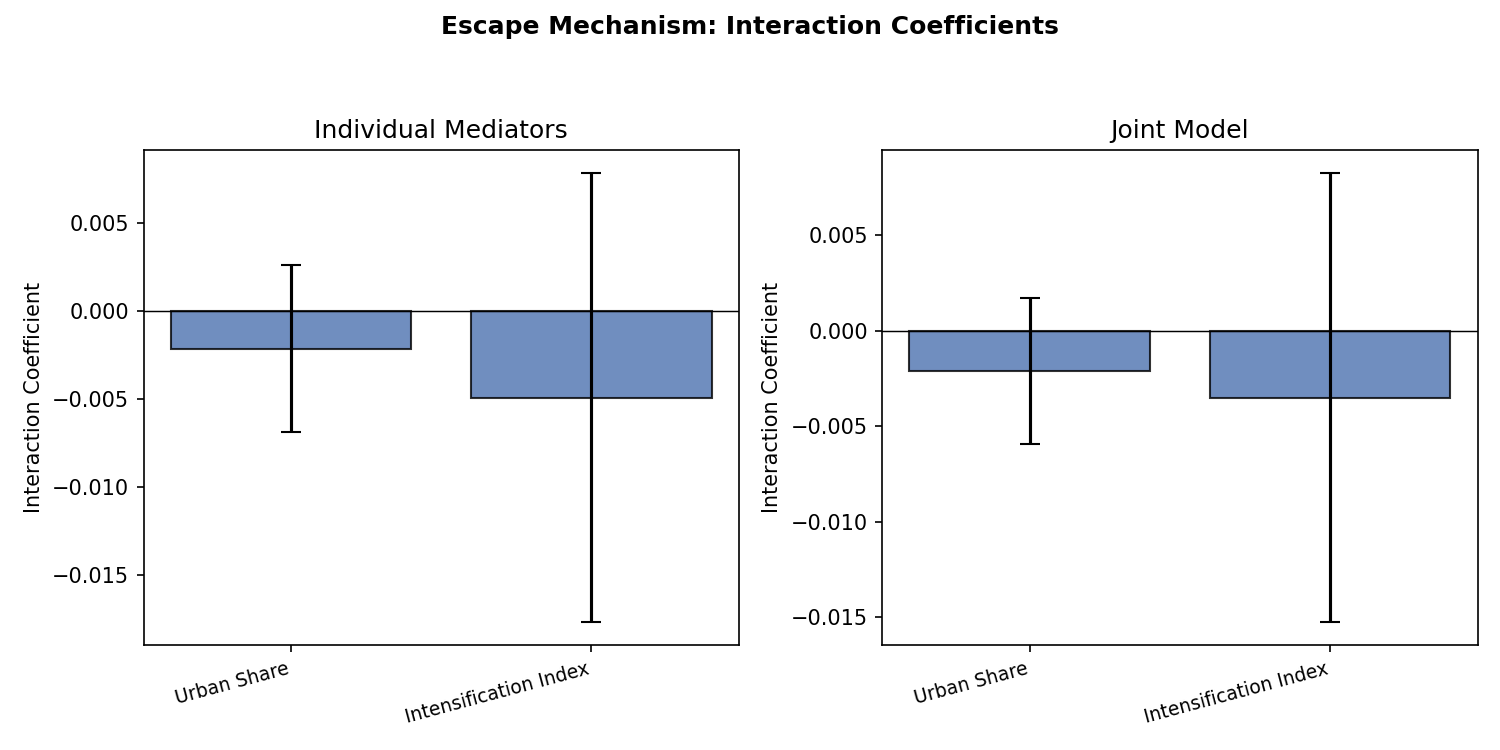
\includegraphics[width=0.6\textwidth]{../analysis/figures/paper4/fig8_escape_mechanism.png}
  \caption{Escape mechanism: interaction coefficients (shock $\times$ mediator) with 95\% confidence intervals. Negative values indicate that the mediator reduces climate sensitivity.}
  \label{fig:escape}
\end{figure}


% ══════════════════════════════════════════════════════════════════════════════
\section{The Long Shadow}
\label{sec:shadow}
% ══════════════════════════════════════════════════════════════════════════════

Does the climate endowment that shaped agricultural systems two millennia ago still matter for modern economic outcomes? We test this by regressing modern (2015--2025 versus 1950--1960) structural changes on pre-industrial (0--1850~CE) seasonality, both with and without pathway fixed effects.

\begin{table}[H]
\centering
\caption{The Long Shadow: Historical Seasonality $\to$ Modern Outcomes}
\label{tab:shadow}
\small
\begin{tabular}{lrrrrr}
\toprule
Outcome & Pathway FE & $\hat{\beta}_{\sigma_s}$ & $p$-value & $R^2$ & $N$ \\
\midrule
$\Delta$ Crop share & No & $-0.425$ & $< 0.001$ & 0.150 & 141 \\
$\Delta$ Crop share & Yes & $-0.466$ & $< 0.001$ & 0.211 & 105 \\
Pop growth (log) & No & $-3.166$ & $< 0.001$ & 0.165 & 141 \\
Pop growth (log) & Yes & $-2.907$ & $< 0.001$ & 0.394 & 105 \\
$\Delta$ Urban share & No & $+0.020$ & $0.084$ & 0.005 & 141 \\
$\Delta$ Irrigation & No & $+0.115$ & $0.079$ & 0.007 & 134 \\
\bottomrule
\end{tabular}
\end{table}

The results are striking. Historical seasonality is a highly significant predictor of modern crop share changes ($\beta = -0.43$, $p < 0.001$) and population growth ($\beta = -3.17$, $p < 0.001$). Higher pre-industrial seasonality is associated with \textit{less} cropland expansion and \textit{lower} population growth in the modern period. This is consistent with the interpretation that high-seasonality regions adopted intensive agriculture early, reached higher density ceilings earlier, and have already undergone the structural transformation toward non-agricultural economies.

Crucially, these effects \textit{survive} the inclusion of pathway fixed effects ($\beta = -0.47$ for crop share, $\beta = -2.91$ for population growth, both $p < 0.001$). This suggests that historical seasonality has persistent effects \textit{beyond} its role in pathway selection---it shapes modern outcomes through channels not fully captured by the pathway typology.

\begin{figure}[H]
  \centering
  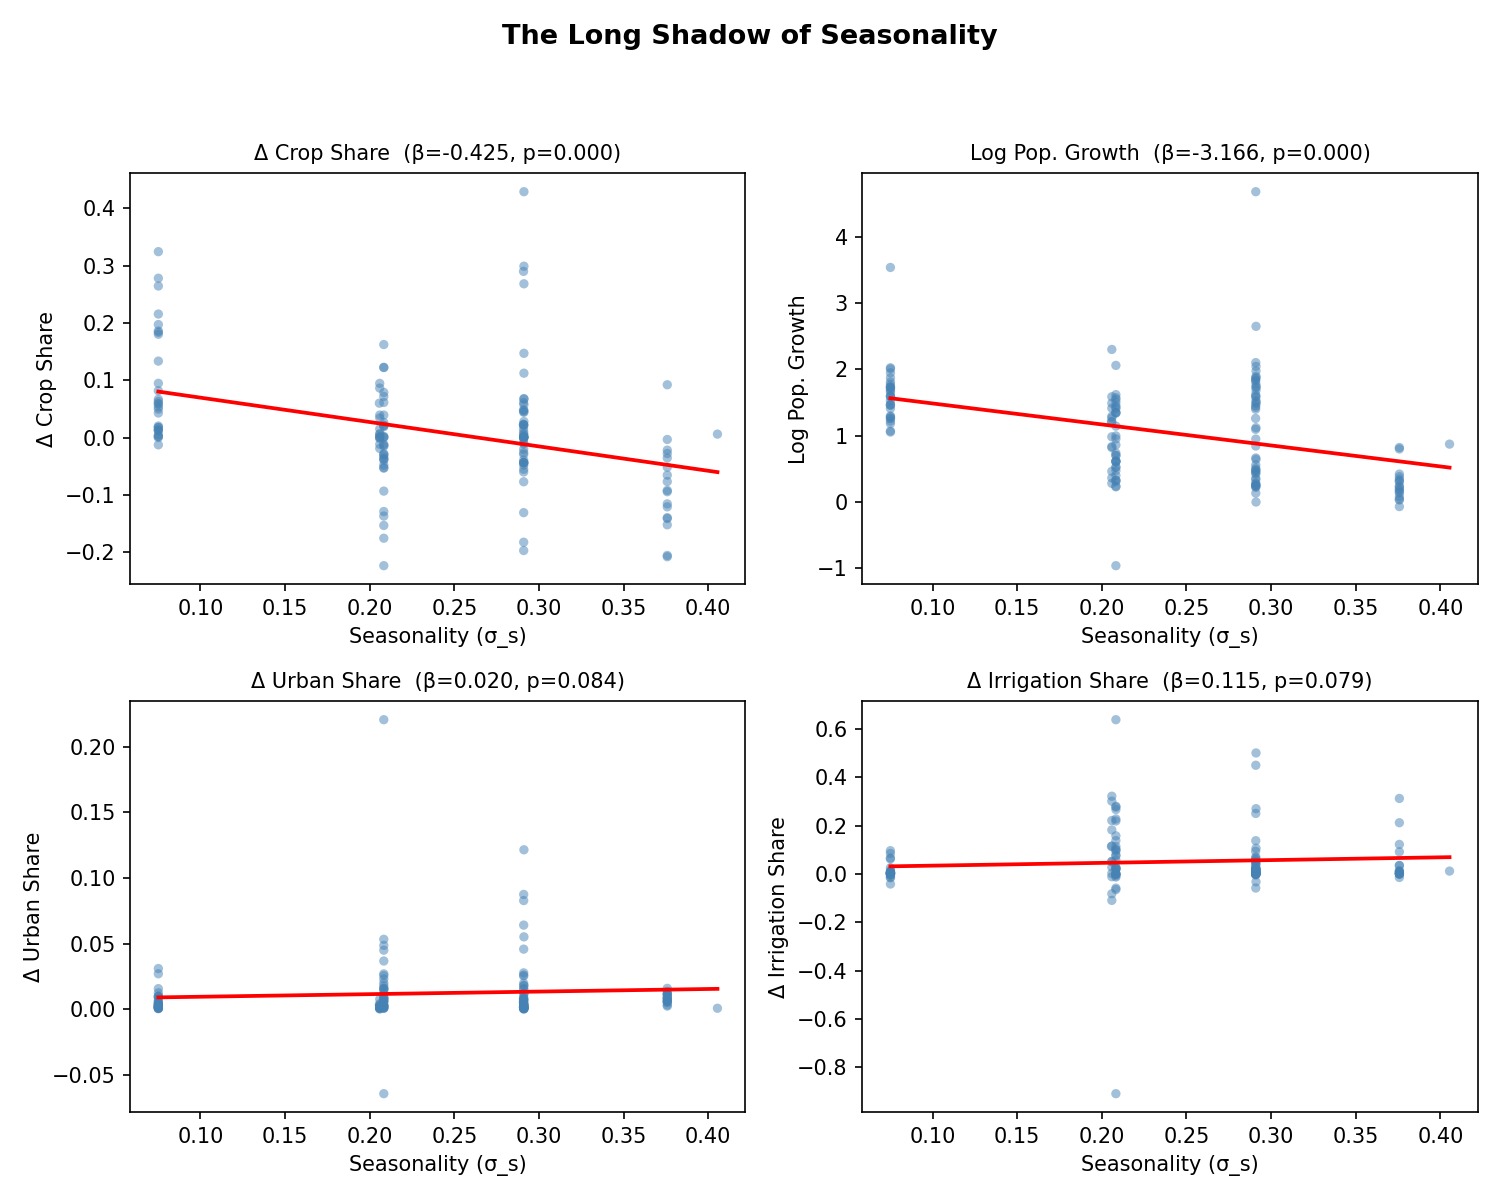
\includegraphics[width=0.85\textwidth]{../analysis/figures/paper4/fig9_long_shadow.png}
  \caption{The long shadow: pre-industrial seasonality (0--1850~CE) versus modern structural outcomes (1950s $\to$ 2015--2025). Each point is a country. OLS regression lines with $\beta$ and $p$-values shown.}
  \label{fig:shadow}
\end{figure}


% ══════════════════════════════════════════════════════════════════════════════
\section{Conclusion}
\label{sec:conclusion}
% ══════════════════════════════════════════════════════════════════════════════

This paper bridges two central literatures in economic growth---the origins of agriculture \citep{matranga2024} and unified growth theory \citep{galor2011unified}---by showing that a single climate endowment shapes the full arc from agricultural adoption through Malthusian dynamics to modern escape.

We make three contributions. First, we develop a two-stage framework in which intra-annual seasonality determines agricultural system selection (Stage~1) and the selected system determines Malthusian dynamics and escape conditions (Stage~2). Second, we construct a 2,000-year calibrated climate panel that enables direct measurement of historical climate variability, improving on the common assumption that modern seasonality approximates ancient conditions. Third, we show that intra-annual seasonality and inter-annual volatility operate through separate causal channels---seasonality drives system selection, volatility drives climate sensitivity---providing a richer account of how climate shapes long-run development.

Our findings have implications for understanding persistent inequality. The ``long shadow'' of seasonality---the finding that pre-industrial climate endowments predict modern structural outcomes even after controlling for agricultural pathway---suggests that climate-determined institutions and technologies have effects that compound over centuries. Societies that adopted intensive agriculture in response to high seasonality not only escaped the Malthusian trap earlier but continue to exhibit different structural dynamics in the modern period.

Several limitations warrant discussion. The PAGES~2k reconstructions provide only decadal/centennial averages, limiting our ability to measure true intra-annual seasonality for historical periods. Our climate panel has 25 regional units for 197 countries, constraining cross-sectional variation in the multinomial logit exercise. The ERA5 coverage is expanding (currently 12 of 25 regions complete) and will substantially improve the precision of modern-period estimates.

These limitations notwithstanding, the central finding is robust: the same climate endowment that determined \textit{which} agricultural system a society adopted also determined \textit{how quickly} that society could escape the Malthusian trap. Seasonality casts a long shadow.


% ══════════════════════════════════════════════════════════════════════════════
% References
% ══════════════════════════════════════════════════════════════════════════════

\bibliographystyle{apalike}

\begin{thebibliography}{99}

\bibitem[Ashraf and Galor(2011)]{ashraf2011dynamics}
Ashraf, Q.~H. and Galor, O. (2011).
\newblock Dynamics of inequality: The role of opportunity and demographics.
\newblock {\em The Quarterly Journal of Economics}, 126(4):2003--2048.

\bibitem[Dell et~al.(2012)]{dell2012temperature}
Dell, M., Jones, B.~F., and Olken, B.~A. (2012).
\newblock Temperature shocks and economic growth: Evidence from the last half century.
\newblock {\em American Economic Journal: Macroeconomics}, 4(3):66--95.

\bibitem[Galor(2011)]{galor2011unified}
Galor, O. (2011).
\newblock {\em Unified Growth Theory}.
\newblock Princeton University Press.

\bibitem[Galor and Weil(2000)]{galor2000population}
Galor, O. and Weil, D.~N. (2000).
\newblock Population, technology, and growth: From Malthusian stagnation to the demographic transition and beyond.
\newblock {\em American Economic Review}, 90(4):806--828.

\bibitem[Goldewijk et~al.(2017)]{goldewijk2017}
Klein~Goldewijk, K., Beusen, A., Doelman, J., and Stehfest, E. (2017).
\newblock Anthropogenic land use estimates for the {H}olocene -- {HYDE} 3.2.
\newblock {\em Earth System Science Data}, 9(2):927--953.

\bibitem[Hersbach et~al.(2020)]{hersbach2020era5}
Hersbach, H., Bell, B., Berrisford, P., et~al. (2020).
\newblock The {ERA5} global reanalysis.
\newblock {\em Quarterly Journal of the Royal Meteorological Society}, 146(730):1999--2049.

\bibitem[Jord\`a(2005)]{jorda2005estimation}
Jord\`a, \`O. (2005).
\newblock Estimation and inference of impulse responses by local projections.
\newblock {\em American Economic Review}, 95(1):161--182.

\bibitem[Manski(2003)]{manski2003partial}
Manski, C.~F. (2003).
\newblock {\em Partial Identification of Probability Distributions}.
\newblock Springer.

\bibitem[Matranga(2024)]{matranga2024}
Matranga, A. (2024).
\newblock The ant and the grasshopper: Seasonality and the invention of agriculture.
\newblock {\em The Quarterly Journal of Economics}, 139(3):1467--1504.

\bibitem[Nunn and Qian(2011)]{nunn2011potato}
Nunn, N. and Qian, N. (2011).
\newblock The potato's contribution to population and urbanization: Evidence from a historical experiment.
\newblock {\em The Quarterly Journal of Economics}, 126(2):593--650.

\end{thebibliography}

\end{document}
